\documentclass[AMA,Times1COL]{WileyNJDv5}

\articletype{Research Article}%

\received{Date Month Year}
\revised{Date Month Year}
\accepted{Date Month Year}
\journal{Statist.\ Med.}
\volume{00}
\copyyear{2025}
\startpage{1}

\raggedbottom

\usepackage{mathtools}
\newcommand{\hnABCD}{\mathrlap{\widehat{\phantom{\text{nA}}}}\text{nABCD}}

\graphicspath{{../figures/}}

\begin{document}

\title{Quantifying Effect Modifier Similarity for Regional Pooling in Multi-Regional Clinical Trials}

\author[1]{Author One}

\author[2]{Author Two}

\author[1]{Author Three}

\authormark{AUTHOR ONE \textsc{et al.}}
\titlemark{QUANTIFYING EFFECT MODIFIER SIMILARITY FOR REGIONAL POOLING}

\address[1]{\orgdiv{Department Name}, \orgname{Institution Name}, \orgaddress{\state{State}, \country{Country}}}

\address[2]{\orgdiv{Department Name}, \orgname{Institution Name}, \orgaddress{\state{State}, \country{Country}}}

\corres{Corresponding Author, Department Name, Institution Name, Address. \email{corresponding@institution.edu}}

\abstract[Abstract]{%
The ICH E17 guideline recommends regional pooling in multi-regional clinical trials (MRCTs) based on similarity of effect modifier distributions, but provides no quantitative methodology. We propose the normalized Area Between Cumulative Distributions (nABCD), a planning-stage dissimilarity index defined as the Wasserstein-1 distance divided by twice the pooled interquartile range. Unlike the standardized mean difference (SMD), nABCD captures differences in variance, shape, and skewness---distributional features that may drive treatment effect heterogeneity through non-linear effect modification. Because nABCD requires only baseline effect modifier distributions, it can be computed from any representative data source, including prior trials, disease registries, and real-world evidence databases---enabling a common planning scenario in which a small-sample region identifies suitable pooling partners before the trial begins. When prior evidence on conditional average treatment effect (CATE) sensitivity is available, clinical calibration translates nABCD into maximum potential regional treatment effect differences ($\Delta_{\max}$) with bootstrap confidence intervals. Simulation studies across eight scenarios demonstrated satisfactory bias and coverage of the percentile bootstrap estimator for non-negligible distributional differences ($\text{nABCD} \geq 0.1$) at $n \geq 100$ per region. Application to two publicly available stroke trial datasets illustrates both common planning scenarios: Case~A (effect modifier unknown; IST-1, 31 countries) using sensitivity analysis, and Case~B (effect modifier identified; IST-3, 8 countries) using clinical calibration. The IST-3 results demonstrate that similar distributional magnitudes can yield markedly different clinical conclusions: NIHSS (nABCD $= 0.240$, $\Delta_{\max} = 5.02$ percentage points) versus age (nABCD $= 0.285$, $\Delta_{\max} = 0.47$ percentage points), underscoring that clinical calibration---not nABCD magnitude alone---should guide pooling decisions. The nABCD framework fills a methodological gap in ICH E17 implementation, supporting evidence-based pooling decisions from any representative population data source.}

\keywords{multi-regional clinical trial; ICH E17; effect modifier; Wasserstein distance; regional pooling; distributional similarity}

\jnlcitation{\cname{%
\author{Author One},
\author{Author Two}, and
\author{Author Three}}.
\ctitle{Quantifying effect modifier similarity for regional pooling in multi-regional clinical trials.} \cjournal{Statist.\ Med.} \cvol{2025;00:1--18}.}

\maketitle

\renewcommand\thefootnote{}
\footnotetext{\textbf{Abbreviations:} ABCD, area between cumulative distributions; CATE, conditional average treatment effect; CDF, cumulative distribution function; CI, confidence interval; EU, European Union; ICH, International Council for Harmonisation; IPD, individual patient data; IQR, interquartile range; IST-3, Third International Stroke Trial; KL, Kullback--Leibler; KS, Kolmogorov--Smirnov; MRCT, multi-regional clinical trial; nABCD, normalized area between cumulative distributions; NIHSS, National Institutes of Health Stroke Scale; NMPA, National Medical Products Administration; OHS, Oxford Handicap Scale; SMD, standardized mean difference; US, United States.}

\renewcommand\thefootnote{\fnsymbol{footnote}}
\setcounter{footnote}{1}

%==============================================================================
\section{Introduction}\label{sec:intro}
%==============================================================================

Multi-regional clinical trials (MRCTs), conducted across multiple countries or regulatory regions under a single protocol, have become the standard paradigm for global pharmaceutical development.\cite{chen2010,quan2010} This approach offers substantial benefits: accelerated timelines, broader generalizability, and earlier access to new therapies for patients worldwide. The International Council for Harmonisation (ICH) E17 guideline, adopted in 2017, established principles for planning and designing MRCTs, with a central assumption that treatment effects are generalizable across the target population.\cite{iche17}

Several regulatory authorities expect demonstration of treatment effect consistency in regional subpopulations,\cite{matsushima2024,song2025} yet individual regional sample sizes in global MRCTs are often insufficient for such demonstration. A key strategy for addressing this challenge is the \emph{regional pooling approach}, wherein regions with similar patient characteristics are grouped for analysis to enhance the ability to assess regional consistency.\cite{iche17} The ICH E17 guideline describes pooling decisions in terms of the similarity of effect modifier distributions.\cite{iche17}

An effect modifier is a baseline patient characteristic---such as age, disease severity, or genetic marker---for which the treatment benefit differs across subgroups. For example, if younger patients respond better to treatment than older patients, age is an effect modifier. When such heterogeneity exists, even if the drug works identically at the individual level, regions with different patient compositions may observe different average treatment effects. A region with predominantly younger patients would show larger benefits than a region with predominantly older patients, not because the drug works differently, but because the patient mix differs. This fundamental relationship underscores why effect modifier distributional similarity is critical to the validity of regional pooling.

Despite the regulatory importance of effect modifier distributional similarity, current practice lacks a standardized quantitative methodology. The ICH E17 guideline provides no specific metric, threshold, or statistical procedure for determining when distributions are ``similar enough.'' Recent regulatory guidance has highlighted this gap. Song et al., writing from the China NMPA perspective on ICH E17 implementation, note the challenge of operationalizing pooling criteria without quantitative tools.\cite{song2025} Long et al.\ further discuss basic considerations for consistency evaluation under ICH E17.\cite{long2025}

This absence of quantitative tools is particularly acute at the \emph{planning stage}, when sponsors must identify suitable pooling partners for small-sample regions. The pooling rationale requires quantitative evidence that partner regions' patient populations are ``similar enough,'' yet no established method exists to provide such evidence. A workshop report by Matsushima et al.\ documented that regional imbalance in CRP-positive/MRI-negative status contributed to apparent inconsistency in the secukinumab MRCT.\cite{matsushima2024} This example illustrates the practical consequences when effect modifier distributional differences are not assessed quantitatively at the planning stage.

Although general-purpose comparison tools such as the standardized mean difference are routinely applied to baseline covariates,\cite{austin2011} they were not designed for assessing effect modifier distributional similarity across regions. As a single summary measure, the standardized mean difference cannot detect differences in variance or distributional shape. When effect modification is non-linear, these distributional features directly influence regional average treatment effects, and a comparison based on means alone will miss them.

This paper addresses these gaps by proposing the \emph{normalized Area Between Cumulative Distributions} (nABCD) as a quantitative index for assessing effect modifier distributional similarity across regions. nABCD is defined as the Wasserstein-1 distance between two cumulative distribution functions, normalized by a robust scale measure (the pooled interquartile range) to achieve scale-free interpretation. Unlike the standardized mean difference, nABCD captures differences in variance and shape simultaneously. We estimate nABCD with bootstrap confidence intervals and link it to clinical interpretation through a calibration framework. We focus on continuous effect modifiers, for which the Wasserstein distance provides a theoretically grounded measure of distributional dissimilarity.

The remainder of this paper is organized as follows. Section~\ref{sec:methods} presents the methodological framework, including the index definition, clinical calibration, and estimation procedure. Section~\ref{sec:simulation} describes a simulation study. Section~\ref{sec:application} demonstrates the framework using publicly available individual patient data. Section~\ref{sec:discussion} discusses implications, limitations, and future directions.

%==============================================================================
\section{Methods}\label{sec:methods}
%==============================================================================

An effect modifier is a factor for which the treatment effect varies across subgroups. Formally, let the conditional average treatment effect (CATE) be denoted $\tau(x) = E[Y(1) - Y(0) \mid X = x]$, where $X$ is the effect modifier. When this function is non-constant, the average treatment effect observed in region $r$ depends on the distribution $F_r$ of the effect modifier in that region:
\begin{equation}
\bar{\tau}_r = \int \tau(x) \, dF_r(x).
\label{eq:regional_ate}
\end{equation}
Assessing pooling suitability therefore requires a measure of distributional difference between regions.

\subsection{Existing Approaches and Their Limitations}\label{sec:existing}

The most widely used measure for comparing covariate distributions across groups is the standardized mean difference (SMD), defined as
\begin{equation}
\text{SMD} = \frac{\bar{X}_1 - \bar{X}_2}{S_{\text{pooled}}},
\label{eq:smd}
\end{equation}
where $\bar{X}_r$ denotes the sample mean in region $r$ and $S_{\text{pooled}}$ is the pooled standard deviation.\cite{austin2011} Because treatment effects in clinical trials are typically summarized as mean differences, SMD provides a scale-free comparison directly relevant to the quantities that drive clinical decision-making. However, by construction SMD captures only differences in location: two distributions with identical means but markedly different variances---for example, $N(50, 5^2)$ and $N(50, 15^2)$---yield $\text{SMD} = 0$ despite a threefold difference in spread.

Distributional distance measures address this limitation by comparing distributions beyond summary statistics. Empirical distribution function (EDF) tests such as the Kolmogorov--Smirnov (KS) statistic, $D_{\text{KS}} = \sup_x |F_1(x) - F_2(x)|$, and related measures (Cram\'{e}r--von Mises, Anderson--Darling) quantify differences in the full shape of distributions by comparing CDFs directly. Information-theoretic divergences such as Kullback--Leibler (KL) divergence,
\begin{equation}
D_{\text{KL}}(P \| Q) = \int p(x) \log \frac{p(x)}{q(x)} \, dx,
\label{eq:kl}
\end{equation}
take a density-based approach, measuring how one probability distribution differs from another.

However, each of these approaches has limitations when applied to comparing effect modifier distributions across regions. SMD captures only location differences and is blind to variance and shape. EDF-based statistics such as the KS statistic capture full distributional differences but lack a clinically interpretable scale and have no theoretical connection to treatment effect heterogeneity. KL divergence is asymmetric---comparing region A to region B yields a different value than comparing B to A---can diverge to infinity when empirical distributions do not fully overlap, and requires density estimation that is impractical with small regional samples. Crucially, none of these measures offers a theoretical link that would translate a distributional distance into a bound on regional treatment effect differences. These gaps motivate a measure that (i) captures distributional features beyond location, (ii) provides a clinically interpretable scale, and (iii) offers such a theoretical link. The nABCD index, defined in the following subsection, is designed to satisfy all three requirements.

\subsection{The nABCD Dissimilarity Index}\label{sec:nabcd_metric}

Among distributional distances that could satisfy these three requirements, we adopt the Wasserstein-1 distance ($W_1$) for its unique theoretical connection to treatment effect heterogeneity (Proposition~\ref{prop:heterogeneity} below). The $W_1$ distance (sometimes called the Earth Mover's Distance) between two cumulative distribution functions $F$ and $G$ is defined as:\cite{villani2009}
\begin{equation}
W_1(F, G) = \int_{-\infty}^{\infty} |F(x) - G(x)| \, dx.
\label{eq:wasserstein}
\end{equation}
Geometrically, this equals the total area between the two CDFs (Figure~\ref{fig:nabcd_definition}). Unlike the standardized mean difference, the Wasserstein distance responds to changes in variance, skewness, and other distributional features.\cite{panaretos2019}

\begin{figure}[t]
\centerline{
\includegraphics[width=\textwidth]{fig2_nabcd_definition.pdf}}
\caption{nABCD as the area between cumulative distribution functions. The shaded region represents the Wasserstein-1 distance $W_1(F_1, F_2)$, which equals the total area between the two CDFs. nABCD normalizes this area by twice the pooled IQR to achieve scale-free interpretation.\label{fig:nabcd_definition}}
\end{figure}

The \emph{normalized Area Between Cumulative Distributions} (nABCD) is defined as the Wasserstein-1 distance normalized by twice the pooled interquartile range:
\begin{equation}
\text{nABCD}(F_1, F_2) = \frac{W_1(F_1, F_2)}{2 \cdot \text{IQR}_{\text{pooled}}},
\label{eq:nabcd}
\end{equation}
where $\text{IQR}_{\text{pooled}} = Q_{0.75}(F_{\text{pool}}) - Q_{0.25}(F_{\text{pool}})$ with $F_{\text{pool}} = \lambda F_1 + (1-\lambda) F_2$ and $\lambda = n_1/(n_1+n_2)$. The denominator normalizes $W_1$ by a scale estimator to achieve scale-free interpretation. We adopt the interquartile range (IQR) for its direct interpretability as the central 50\% spread of the effect modifier distribution. The factor of 2 calibrates nABCD so that a one-IQR location shift yields nABCD $= 0.5$.

$W_1$ is a proper distance satisfying the triangle inequality.\cite{villani2009} Normalization by the pair-dependent pooled IQR does not preserve this property, but it enables comparison of distributional similarity across effect modifiers measured on different scales---a practical necessity when assessing multiple covariates simultaneously. nABCD thus serves as a dissimilarity index retaining non-negativity, symmetry, and identity of indiscernibles (Proposition~\ref{prop:nonnegativity}).

\begin{proposition}\label{prop:nonnegativity}
\textup{(Non-negativity).} For distributions with finite first moment, provided $\mathrm{IQR}_{\mathrm{pooled}} > 0$ (i.e., the pooled distribution is non-degenerate), $\text{nABCD} \geq 0$, with equality if and only if $F_1 = F_2$.
\end{proposition}

The specific choice of $W_1$ as the underlying distance is motivated by the Kantorovich--Rubinstein duality theorem,\cite{villani2009} which provides a theoretical bridge between distributional distance and treatment effect heterogeneity. The connection proceeds in three steps:
\begin{enumerate}[1.]
\item \emph{$W_1$ as CDF area}: In one dimension, $W_1(F_1, F_2) = \int |F_1(x) - F_2(x)| \, dx$ (equation~\ref{eq:wasserstein}), the total area between two CDFs. This area increases whenever the distributions differ in location, spread, or shape.
\item \emph{Kantorovich--Rubinstein duality}: The $W_1$ distance has an equivalent dual representation:\cite{villani2009}
\[
W_1(F_1, F_2) = \sup_{\|f\|_{\text{Lip}} \leq 1} \left|\int f \, dF_1 - \int f \, dF_2\right|.
\]
That is, $W_1$ equals the largest possible difference in expected values of $f$ between the two distributions, where the supremum is taken over all functions whose rate of change is bounded by~1 ($|f(x) - f(y)| \leq |x - y|$ for all $x, y$; such functions are called 1-Lipschitz).
\item \emph{CATE application}: A function is Lipschitz continuous with constant $L$ if its rate of change is bounded by $L$: $|\tau(x) - \tau(y)| \leq L|x - y|$ for all $x, y$. In clinical terms, $L$ controls how much the treatment effect can change per unit change in the effect modifier. Since $\tau/L$ is 1-Lipschitz, applying the duality yields:
\end{enumerate}
\begin{equation}
|\bar{\tau}_1 - \bar{\tau}_2| \leq L \cdot W_1(F_1, F_2).
\label{eq:heterogeneity_bound}
\end{equation}
This Lipschitz-dual characterization is specific to $W_1$. The $W_2$ distance, while admitting closed-form expressions for Gaussian families, does not possess it and therefore cannot provide such a bound. The alternative measures discussed in Section~\ref{sec:existing} similarly lack any analogous property.\cite{gibbs2002}

Combining the bound above with the nABCD definition (equation~\ref{eq:nabcd}) yields the central result:

\begin{proposition}\label{prop:heterogeneity}
\textup{(Connection to heterogeneity).} If the CATE function is Lipschitz continuous with constant $L$, then
\begin{equation}
|\bar{\tau}_1 - \bar{\tau}_2| \leq 2L \cdot \text{IQR}_{\textup{pooled}} \cdot \text{nABCD}(F_1, F_2).
\label{eq:heterogeneity_nabcd}
\end{equation}
\end{proposition}

\begin{proof}
Substituting (\ref{eq:nabcd}) into (\ref{eq:heterogeneity_bound}) yields $|\bar{\tau}_1 - \bar{\tau}_2| \leq L \cdot W_1(F_1, F_2) = L \cdot 2 \cdot \text{IQR}_{\text{pooled}} \cdot \text{nABCD}(F_1, F_2) = 2L \cdot \text{IQR}_{\text{pooled}} \cdot \text{nABCD}(F_1, F_2)$.
\end{proof}

\noindent The Lipschitz assumption is appropriate when the CATE function varies smoothly with the effect modifier. For threshold or step-function CATEs, $L$ can be arbitrarily large and the bound becomes conservative; in such cases the clinical calibration should be interpreted as a worst-case bound rather than a tight estimate (see Section~\ref{sec:discussion}).

\subsection{Estimation}\label{sec:estimation}

Given samples $\{X_{1,i}\}_{i=1}^{n_1}$ from region 1 and $\{X_{2,j}\}_{j=1}^{n_2}$ from region 2, nABCD is estimated using empirical distribution functions. Since $\hat{F}_1$ and $\hat{F}_2$ are piecewise constant (right-continuous step functions), the integral in equation~(\ref{eq:wasserstein}) reduces to a finite sum over the intervals defined by the combined order statistics:
\begin{equation}
\hnABCD = \frac{\sum_{k=1}^{n_1+n_2-1} |\hat{F}_1(x_{(k)}) - \hat{F}_2(x_{(k)})| \cdot (x_{(k+1)} - x_{(k)})}{2 \cdot \widehat{\text{IQR}}_{\text{pooled}}},
\label{eq:estimator}
\end{equation}
where $\hat{F}_r$ denotes the empirical CDF (right-continuous) of region $r$, and $x_{(1)} < \cdots < x_{(n_1+n_2)}$ are the combined order statistics. The asymptotic distribution of $W_1$ is non-standard: del Barrio et al.\cite{delbarrio1999} showed that $\sqrt{n}\,W_1(\hat{F}_n, F) \xrightarrow{d} \int |B(F(x))|\,dx$, where $B$ is a standard Brownian bridge. Because the quantiles of this limiting distribution depend on the unknown $F$, no universal critical values are available and direct construction of asymptotic confidence intervals is impractical. We therefore employ the nonparametric percentile bootstrap with $B = 2{,}000$ replicates.\cite{efron1993} In the two-sample setting, when $F_1 \neq F_2$ the Hadamard derivative of the $L_1$ functional is linear, so the ordinary nonparametric bootstrap is consistent;\cite{sommerfeld2018} convergence occurs at rate $\sqrt{n_1 n_2/(n_1+n_2)}$ (see Appendix~\ref{app:asymptotic} for details). The estimator~(\ref{eq:estimator}) is computed in $O((n_1 + n_2) \log(n_1 + n_2))$ time, dominated by sorting the combined order statistics.

\subsection{Interpretation and Clinical Calibration}\label{sec:inference}

A central feature of nABCD is its connection to treatment effect heterogeneity through Proposition~\ref{prop:heterogeneity}. This connection provides the basis for a clinically grounded interpretation framework rather than reliance on fixed thresholds alone.

\subsubsection{Clinical Calibration via the Heterogeneity Bound}

From equation~(\ref{eq:heterogeneity_nabcd}), the maximum potential difference in regional average treatment effects attributable to effect modifier distributional differences is:
\begin{equation}
\Delta_{\max} = 2L \cdot \text{IQR}_{\text{pooled}} \cdot \text{nABCD}(F_1, F_2),
\label{eq:delta_max}
\end{equation}
where $L$ is the Lipschitz constant of the CATE function $\tau(x)$ with respect to the effect modifier. $L$ serves as a sensitivity parameter controlling the worst-case treatment effect heterogeneity, and can be estimated from prior knowledge, pilot data, or published subgroup analyses.

The clinical calibration procedure is as follows:
\begin{enumerate}[1.]
\item Identify candidate effect modifiers and compute nABCD with bootstrap CIs for each effect modifier across region pairs.
\item For each effect modifier, estimate or bound $L$ from prior knowledge (e.g., subgroup analyses showing treatment effect varies by $\Delta\tau$ per unit change in the effect modifier, giving $L \approx \Delta\tau / \Delta x$).
\item Compute $\Delta_{\max}$ using equation~(\ref{eq:delta_max}). This represents the worst-case treatment effect difference attributable to the distributional difference.
\item Derive the bootstrap CI for $\Delta_{\max}$ from the nABCD confidence interval: $[\Delta_{\max,L},\, \Delta_{\max,U}] = 2L \cdot \text{IQR}_{\text{pooled}} \cdot [\text{nABCD}_{L},\, \text{nABCD}_{U}]$. This expresses inferential uncertainty directly on the clinical scale.
\item Report $\Delta_{\max}$ and its CI alongside the clinical context---for example, the overall treatment effect size, the non-inferiority margin, or the minimal clinically important difference. This information enables trial designers and regulatory scientists to exercise clinical judgment about pooling, considering the totality of evidence rather than a binary accept/reject decision.
\end{enumerate}

This estimation-centered approach deliberately avoids forcing pooling decisions into a binary hypothesis testing framework. The rationale is threefold. First, the ICH E17 guideline describes ``similar enough'' as inherently context-dependent, and reducing this judgment to a rejection threshold risks oversimplification. Second, the uncertainty in $L$ means that $\Delta_{\max}$ itself is subject to sensitivity analysis (Section~\ref{sec:application}); a binary test cannot naturally accommodate this layered uncertainty. Third, consistent with recent calls to move beyond dichotomous statistical decisions,\cite{wasserstein2016} presenting $\Delta_{\max}$ with its CI provides richer information for regulatory deliberation than a p-value or a reject/fail-to-reject outcome.

When regulatory agencies require a formal decision rule, the estimation framework can be adapted: declare pooling acceptable if the upper bound of the 95\% CI for $\Delta_{\max}$ falls below a pre-specified clinical margin $\Delta_{\text{clin}}$. However, we recommend this as a supplementary rather than primary use of the nABCD framework.

The clinical calibration procedure is demonstrated with real clinical trial data in Section~\ref{sec:application}, where two candidate effect modifiers with contrasting levels of CATE sensitivity evidence illustrate both full calibration and planning-stage assessment workflows.

\subsubsection{Sensitivity Analysis When $L$ Is Unknown}\label{sec:sensitivity}

When $L$ cannot be estimated from prior data---the most common situation at the MRCT planning stage---the clinical calibration framework supports two complementary approaches. First, the reference benchmarks (Table~\ref{tab:benchmarks}) provide an initial assessment of distributional magnitude without requiring $L$. Second, a reverse sensitivity analysis asks: \emph{what value of $L$ would be required for a given nABCD to produce a clinically meaningful $\Delta_{\max}$?} Rearranging equation~(\ref{eq:delta_max}):
\begin{equation}
L^* = \frac{\Delta_{\text{clin}}}{2 \cdot \text{IQR}_{\text{pooled}} \cdot \text{nABCD}},
\label{eq:lstar}
\end{equation}
where $\Delta_{\text{clin}}$ is a pre-specified clinically important treatment effect difference (e.g., the overall treatment effect or the non-inferiority margin). If $L^*$ exceeds the largest plausible CATE sensitivity for the effect modifier under consideration, the distributional difference is unlikely to produce meaningful treatment effect heterogeneity, regardless of the true $L$. This reverse calculation is demonstrated in Case~A of Section~\ref{sec:application}.

\subsubsection{Reference Benchmarks}

When prior knowledge of $L$ is unavailable, the benchmarks in Table~\ref{tab:benchmarks} provide a convenience reference for initial assessment. These labels describe \emph{distributional magnitude} only and should not be conflated with clinical significance: as the calibration framework (equation~\ref{eq:delta_max}) and Section~\ref{sec:application} demonstrate, a ``large'' nABCD for a weak effect modifier may carry less clinical consequence than a ``moderate'' nABCD for a strong effect modifier, because CATE sensitivity $L$ determines how distributional distance translates into treatment effect heterogeneity.

\begin{table}[ht]
\caption{Reference benchmarks for nABCD values when CATE sensitivity $L$ is unknown.\label{tab:benchmarks}}
\begin{tabular*}{\textwidth}{@{\extracolsep\fill}lll@{}}
\toprule
\textbf{nABCD Range} & \textbf{Distributional Magnitude} & \textbf{Calibration Guidance} \\
\midrule
$< 0.05$ & Negligible & Clinical calibration unlikely to reveal meaningful $\Delta_{\max}$ \\
$0.05$--$0.15$ & Small & Calibration recommended if $L$ is available \\
$0.15$--$0.30$ & Moderate & Calibration important; interpret in clinical context \\
$> 0.30$ & Large & Calibration essential before pooling deliberation \\
\bottomrule
\end{tabular*}
\begin{tablenotes}
\item These benchmarks serve as initial reference points only; clinical interpretation should always proceed through the calibration framework of Section~\ref{sec:inference}, as the same nABCD value may have different clinical implications depending on the Lipschitz constant $L$. Under Gaussian location shift, the benchmark boundaries correspond approximately to SMD $= 0.2$, $0.5$, and $1.0\sigma$ (simulation scenarios S2, S3, and S4 in Table~\ref{tab:scenarios}, with true nABCD values of 0.073, 0.180, and 0.328 respectively). Actual pooling decisions should use clinical calibration (equation~\ref{eq:delta_max}) whenever possible.
\end{tablenotes}
\end{table}

%==============================================================================
\section{Simulation Study}\label{sec:simulation}
%==============================================================================

We conducted simulation studies to evaluate the estimation properties of the nABCD estimator: bias, variability, and coverage probability of bootstrap confidence intervals. These properties are essential for the clinical calibration framework, as reliable estimation of nABCD directly determines the quality of $\Delta_{\max}$ estimates. We assessed performance across a range of scenarios relevant to MRCT applications.

\subsection{Simulation Design}\label{sec:sim_design}

\subsubsection{Scenarios}

We designed eight systematic scenarios for methodological validation, examining controlled distributional differences across location, scale, shape, and combinations thereof. Table~\ref{tab:scenarios} summarizes these scenarios with their true nABCD values.

\begin{table}[ht]
\caption{Simulation scenarios with clinical motivations.\label{tab:scenarios}}
\begin{tabular*}{\textwidth}{@{\extracolsep\fill}lllll@{}}
\toprule
\textbf{ID} & \textbf{Description} & \textbf{Distribution 1} & \textbf{Distribution 2} & \textbf{True nABCD} \\
\midrule
S1 & Null (identical) & $N(50, 10^2)$ & $N(50, 10^2)$ & 0.000 \\
S2 & Location 0.2$\sigma$ & $N(50, 10^2)$ & $N(52, 10^2)$ & 0.073 \\
S3 & Location 0.5$\sigma$ & $N(50, 10^2)$ & $N(55, 10^2)$ & 0.180 \\
S4 & Location 1.0$\sigma$ & $N(50, 10^2)$ & $N(60, 10^2)$ & 0.328 \\
S5 & Scale 1.5$\times$ & $N(50, 10^2)$ & $N(50, 15^2)$ & 0.122 \\
S6 & Shape (Gamma) & $N(50, 10^2)$ & Gamma$(25, 0.5)$ & 0.024 \\
S7 & Skew (Log-normal) & $N(50, 10^2)$ & LogN$(\mu, \sigma)$ & 0.304 \\
S8 & Location + Scale & $N(50, 10^2)$ & $N(55, 15^2)$ & 0.175 \\
\bottomrule
\end{tabular*}
\begin{tablenotes}
\item The Gamma distribution in S6 has shape parameter 25 and rate 0.5, yielding mean 50 and standard deviation 10. The Log-normal in S7 is parameterized to match mean 50 with CV $\approx$ 53\%, typical of clinical biomarkers such as ALT. S8 combines location and scale differences, representing the most realistic MRCT pattern.
\end{tablenotes}
\end{table}

\subsubsection{Simulation Parameters}

For each scenario, we generated samples of size $n = 50$, 100, and 200 per region, reflecting sample sizes typical in MRCT regional subgroups. We performed 10{,}000 replications per scenario--sample size combination to ensure stable estimates of operating characteristics, with Monte Carlo standard errors below 0.005 for all reported proportions. Bootstrap confidence intervals were computed using $B = 2{,}000$ resamples. All simulations were conducted in R version 4.5.1. True nABCD values for all scenarios were computed via Monte Carlo integration ($n_{\textup{MC}} = 10^6$) using the mixture IQR, avoiding closed-form approximations that may use component rather than pooled IQR.

\subsubsection{Evaluation Metrics}

Consistent with the estimation-centered framework, we evaluated:
\begin{enumerate}[1.]
\item \emph{Bias}: $\text{Mean}(\hnABCD) - \text{nABCD}$
\item \emph{Root mean squared error (RMSE)}: $\sqrt{\text{Mean}[(\hnABCD - \text{nABCD})^2]}$
\item \emph{Coverage probability}: Proportion of 95\% bootstrap CIs containing the true value
\item \emph{CI width}: Mean width of bootstrap CIs, reflecting estimation precision
\end{enumerate}

\subsection{Results}\label{sec:sim_results}

\subsubsection{Point Estimation and Coverage}

Table~\ref{tab:bias} presents the bias of the nABCD estimator across scenarios and sample sizes. The estimator showed positive bias under the null hypothesis (S1), with bias decreasing from 0.093 at $n=50$ to 0.047 at $n=200$. This positive bias is attributable to the non-negative nature of the Wasserstein distance: even when true nABCD equals zero, sampling variability produces positive estimates.

\begin{table}[ht]
\caption{Bias of nABCD estimator by scenario and sample size.\label{tab:bias}}
\begin{tabular*}{\textwidth}{@{\extracolsep\fill}lcccc@{}}
\toprule
\textbf{Scenario} & \textbf{True nABCD} & $\boldsymbol{n=50}$ & $\boldsymbol{n=100}$ & $\boldsymbol{n=200}$ \\
\midrule
S1 (Null) & 0.000 & 0.093 & 0.066 & 0.047 \\
S2 (0.2$\sigma$) & 0.073 & 0.039 & 0.020 & 0.009 \\
S3 (0.5$\sigma$) & 0.180 & 0.010 & 0.003 & 0.001 \\
S4 (1.0$\sigma$) & 0.328 & 0.006 & 0.003 & 0.001 \\
S5 (Scale) & 0.122 & 0.028 & 0.014 & 0.007 \\
S6 (Shape) & 0.024 & 0.071 & 0.046 & 0.028 \\
S7 (Skew) & 0.304 & 0.015 & 0.008 & 0.003 \\
S8 (Loc+Scale) & 0.175 & 0.023 & 0.011 & 0.006 \\
\bottomrule
\end{tabular*}
\begin{tablenotes}
\item Bias is defined as $\text{Mean}(\hnABCD) - \text{nABCD}$. Results based on 10{,}000 replications with $B = 2{,}000$ bootstrap resamples.
\end{tablenotes}
\end{table}

For scenarios with true nABCD above approximately 0.1, bias was less than 0.02 in absolute value at $n \geq 100$, indicating satisfactory point estimation performance at practical sample sizes (Figure~\ref{fig:bias}). For S4 (1.0$\sigma$ location shift), bias was negligible (0.006 at $n=50$, 0.001 at $n=200$), confirming accurate estimation even for large distributional differences. For scenarios near the boundary (S1, S2, S6), positive bias was more pronounced and diminished slowly with sample size---a well-known phenomenon for non-negative statistics where sampling variability inflates estimates when the true value is close to zero. S6 (shape) exhibited the largest bias among non-null scenarios (0.071 at $n=50$, 0.028 at $n=200$), because its true nABCD (0.024) lies in the near-boundary regime where the non-negativity constraint dominates.

\begin{figure}[t]
\centerline{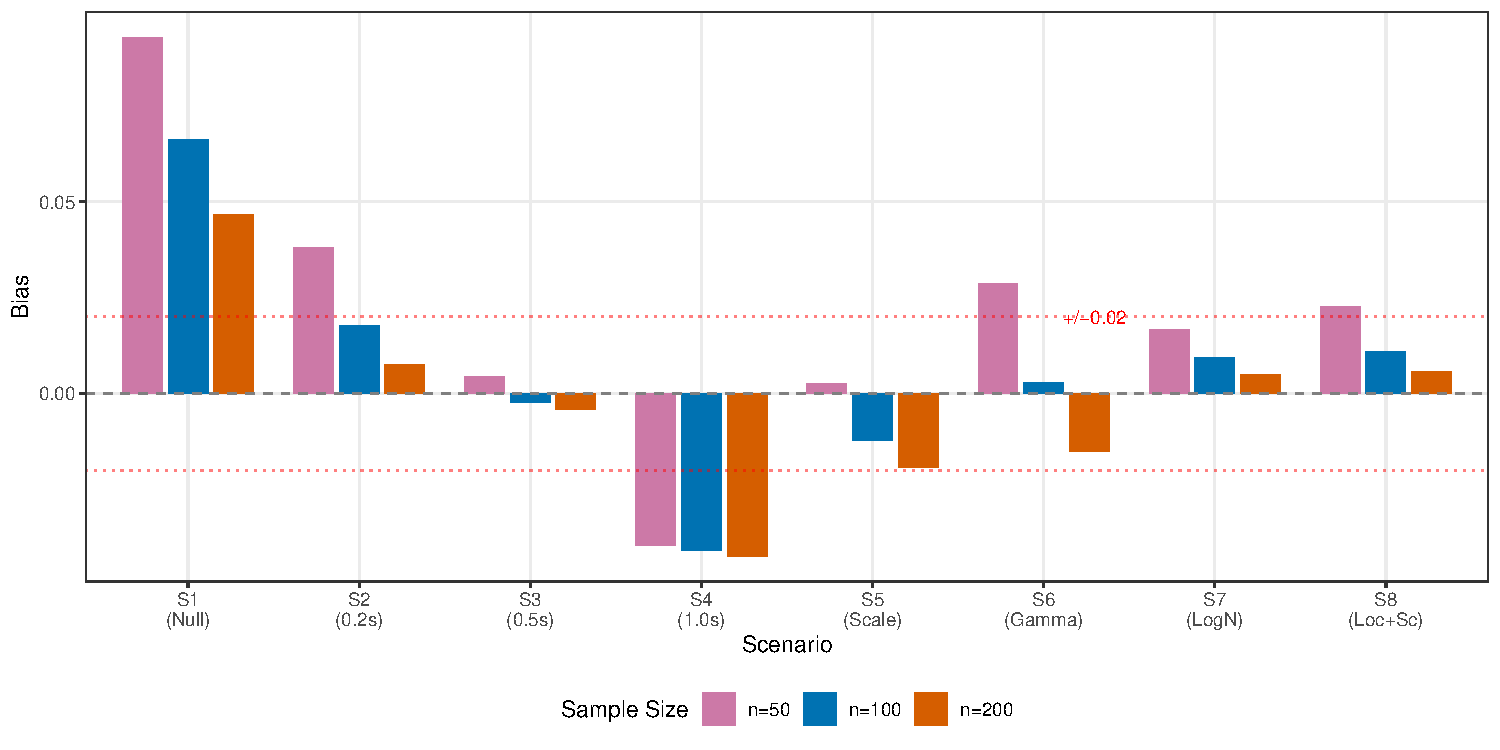
\includegraphics[width=\textwidth]{fig3_bias.pdf}}
\caption{Bias of nABCD estimator by scenario and sample size. Horizontal dashed lines indicate $\pm 0.02$ bias threshold. For scenarios with true nABCD above 0.1, bias is less than 0.02 at $n \geq 100$. Near-boundary scenarios (S1, S6) show larger positive bias due to the non-negativity constraint.\label{fig:bias}}
\end{figure}

Table~\ref{tab:coverage} presents coverage probabilities of the 95\% bootstrap confidence intervals. For scenarios with true nABCD above approximately 0.1, coverage was near-nominal at $n \geq 100$: S3 (0.947--0.951), S4 (0.950--0.957), S7 (0.953--0.954), and S8 (0.935--0.944). S4 (1.0$\sigma$ location shift) showed particularly stable coverage across all sample sizes, with no degradation at larger $n$, confirming satisfactory bootstrap performance even for large distributional differences. S5 (scale) showed moderate undercoverage at $n=50$ (0.856) that improved to near-nominal at $n=200$ (0.933). S2 (small location shift) showed undercoverage at $n=50$ (0.652) due to its near-boundary true value, improving to 0.941 at $n=200$.

Coverage for S6 (shape) is not reported because its true nABCD (0.024) is sufficiently small that positive bias dominates at all sample sizes considered. This is the same boundary phenomenon observed for S1 (null): when the true value lies near the parameter space boundary, the non-negativity constraint on nABCD produces persistent positive bias that prevents the confidence interval from containing the true value. This does not indicate estimator failure---the estimator is consistent---but rather that sample sizes well beyond 200 per region would be needed for reliable inference when the true distributional difference is negligible.

We also evaluated BCa (bias-corrected and accelerated) confidence intervals in preliminary experiments. BCa intervals showed consistently lower coverage than percentile intervals across all scenarios, particularly for near-boundary scenarios. The BCa correction overcorrects for nABCD because the statistic is bounded below by zero, causing the acceleration parameter to distort the quantile adjustment. Based on these findings, we adopt percentile bootstrap as the primary inference method.

Monte Carlo standard errors for all reported coverage probabilities were below 0.005 at 10{,}000 replications, ensuring that observed differences across scenarios and sample sizes reflect genuine operating characteristic differences rather than simulation noise.

\begin{table}[ht]
\caption{Coverage probability of 95\% percentile bootstrap confidence intervals.\label{tab:coverage}}
\begin{tabular*}{\textwidth}{@{\extracolsep\fill}lccc@{}}
\toprule
\textbf{Scenario} & $\boldsymbol{n=50}$ & $\boldsymbol{n=100}$ & $\boldsymbol{n=200}$ \\
\midrule
S2 (0.2$\sigma$) & 0.652 & 0.881 & 0.941 \\
S3 (0.5$\sigma$) & 0.947 & 0.951 & 0.947 \\
S4 (1.0$\sigma$) & 0.950 & 0.950 & 0.957 \\
S5 (Scale) & 0.856 & 0.910 & 0.933 \\
S7 (Skew) & 0.953 & 0.954 & 0.954 \\
S8 (Loc+Scale) & 0.917 & 0.935 & 0.944 \\
\bottomrule
\end{tabular*}
\begin{tablenotes}
\item Coverage under S1 (Null) and S6 (Shape) is not reported because the true nABCD lies near the boundary of the parameter space (0 and 0.024, respectively), where positive bias from the non-negativity constraint prevents meaningful coverage assessment.
\item For S4, coverage was near-nominal across all sample sizes (0.950--0.957), confirming satisfactory performance even for large distributional differences. The undercoverage for S2 at small sample sizes (0.652 at $n=50$) and S5 (0.856 at $n=50$) reflects boundary proximity effects that diminish with increasing $n$.
\end{tablenotes}
\end{table}

\subsubsection{Estimation Precision}

Figure~\ref{fig:estimation_quality} summarizes the estimation quality across scenarios and sample sizes, presenting both coverage probabilities and mean CI widths.

\begin{figure*}[t]
\centerline{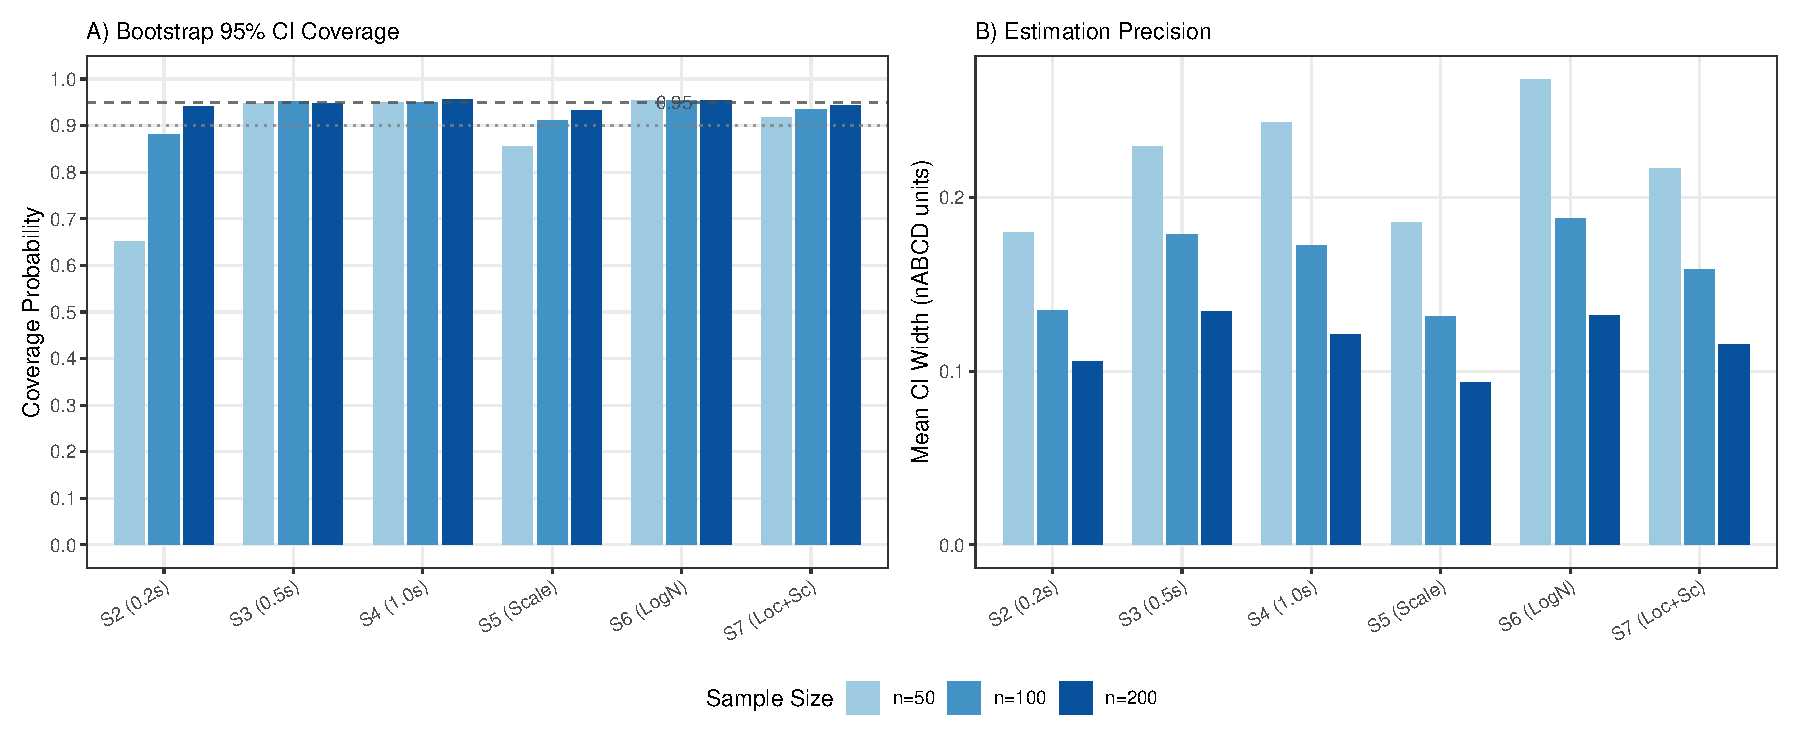
\includegraphics[width=\textwidth]{fig4_estimation_quality.pdf}}
\caption{Estimation quality of nABCD bootstrap inference. Panel~(A) shows coverage probability of 95\% bootstrap confidence intervals; dashed and dotted lines indicate the nominal 0.95 and minimum acceptable 0.90 levels. Panel~(B) shows mean CI width in nABCD units. Coverage exceeds 0.90 for most scenarios at $n \geq 100$; CI width narrows consistently with increasing $n$.\label{fig:estimation_quality}}
\end{figure*}

Table~\ref{tab:precision} presents the RMSE and mean CI width across scenarios. RMSE decreased consistently with increasing $n$, reaching values below 0.05 for all scenarios at $n = 200$ except S6 (shape), where the near-boundary bias inflated RMSE. Mean CI width narrowed proportionally, with CIs at $n = 100$ typically spanning 0.11--0.19 in nABCD units. In the clinical calibration framework, this CI width propagates to $\Delta_{\max}$: for example, with $L = 0.01$/pt and IQR $= 11$ (values representative of NIHSS in the IST-3 application), a CI width of 0.13 in nABCD corresponds to a $\Delta_{\max}$ CI width of $2 \times 0.01 \times 11 \times 0.13 = 0.029$ (2.9\%pt)---a level of precision sufficient for meaningful clinical calibration.

\begin{table}[ht]
\caption{RMSE and mean CI width by scenario and sample size.\label{tab:precision}}
\begin{tabular*}{\textwidth}{@{\extracolsep\fill}lcccccc@{}}
\toprule
& \multicolumn{3}{c}{\textbf{RMSE}} & \multicolumn{3}{c}{\textbf{Mean CI Width}} \\
\cmidrule(lr){2-4}\cmidrule(lr){5-7}
\textbf{Scenario} & $\boldsymbol{n=50}$ & $\boldsymbol{n=100}$ & $\boldsymbol{n=200}$ & $\boldsymbol{n=50}$ & $\boldsymbol{n=100}$ & $\boldsymbol{n=200}$ \\
\midrule
S1 (Null) & 0.099 & 0.069 & 0.049 & 0.16 & 0.11 & 0.08 \\
S2 (0.2$\sigma$) & 0.061 & 0.044 & 0.032 & 0.18 & 0.13 & 0.11 \\
S3 (0.5$\sigma$) & 0.067 & 0.048 & 0.035 & 0.23 & 0.18 & 0.13 \\
S4 (1.0$\sigma$) & 0.062 & 0.043 & 0.030 & 0.24 & 0.17 & 0.12 \\
S5 (Scale) & 0.053 & 0.036 & 0.025 & 0.19 & 0.13 & 0.09 \\
S6 (Shape) & 0.080 & 0.053 & 0.033 & 0.16 & 0.11 & 0.08 \\
S7 (Skew) & 0.070 & 0.049 & 0.034 & 0.27 & 0.19 & 0.13 \\
S8 (Loc+Scale) & 0.062 & 0.043 & 0.030 & 0.22 & 0.16 & 0.12 \\
\bottomrule
\end{tabular*}
\begin{tablenotes}
\item CI width is defined as mean of (upper $-$ lower) across 10{,}000 replications.
\end{tablenotes}
\end{table}

Under the null hypothesis (S1), the positive bias produces CIs that are shifted upward from zero. At $n = 50$, the mean estimate was 0.093 with mean CI width 0.16; at $n = 200$, the mean estimate decreased to 0.047 with mean CI width 0.08. This bias is relevant for clinical calibration: when the true distributional difference is zero, the estimator will suggest a small positive $\Delta_{\max}$. Practitioners should be aware of this conservative tendency, particularly at smaller sample sizes.

\subsubsection{Comparison with Standardized Mean Difference}

Table~\ref{tab:smd} compares the sensitivity of nABCD and SMD to different types of distributional differences. While both metrics respond to location shifts, SMD is insensitive to differences in variance and shape---the very types of distributional differences that may drive treatment effect heterogeneity through non-linear CATE functions.

\begin{table}[ht]
\caption{Sensitivity comparison: nABCD versus SMD at $n=100$.\label{tab:smd}}
\begin{tabular*}{\textwidth}{@{\extracolsep\fill}lccc@{}}
\toprule
\textbf{Scenario} & \textbf{nABCD (mean $\pm$ SD)} & \textbf{SMD (mean $\pm$ SD)} & \textbf{Implication} \\
\midrule
S3 (Location) & $0.183 \pm 0.048$ & $0.50 \pm 0.14$ & Both detect \\
S5 (Scale only) & $0.136 \pm 0.033$ & $0.00 \pm 0.14$ & Only nABCD detects \\
S6 (Shape only) & $0.070 \pm 0.025$ & $0.00 \pm 0.14$ & Only nABCD detects \\
S7 (Skew only) & $0.312 \pm 0.048$ & $0.00 \pm 0.14$ & Only nABCD detects \\
\bottomrule
\end{tabular*}
\begin{tablenotes}
\item SMD depends only on the difference in means, making it insensitive to differences in variance, shape, and skewness. nABCD captures the full distributional difference. S7 is particularly informative: a large distributional difference (nABCD $= 0.31$) is entirely invisible to SMD.
\end{tablenotes}
\end{table}

\begin{figure*}[t]
\centerline{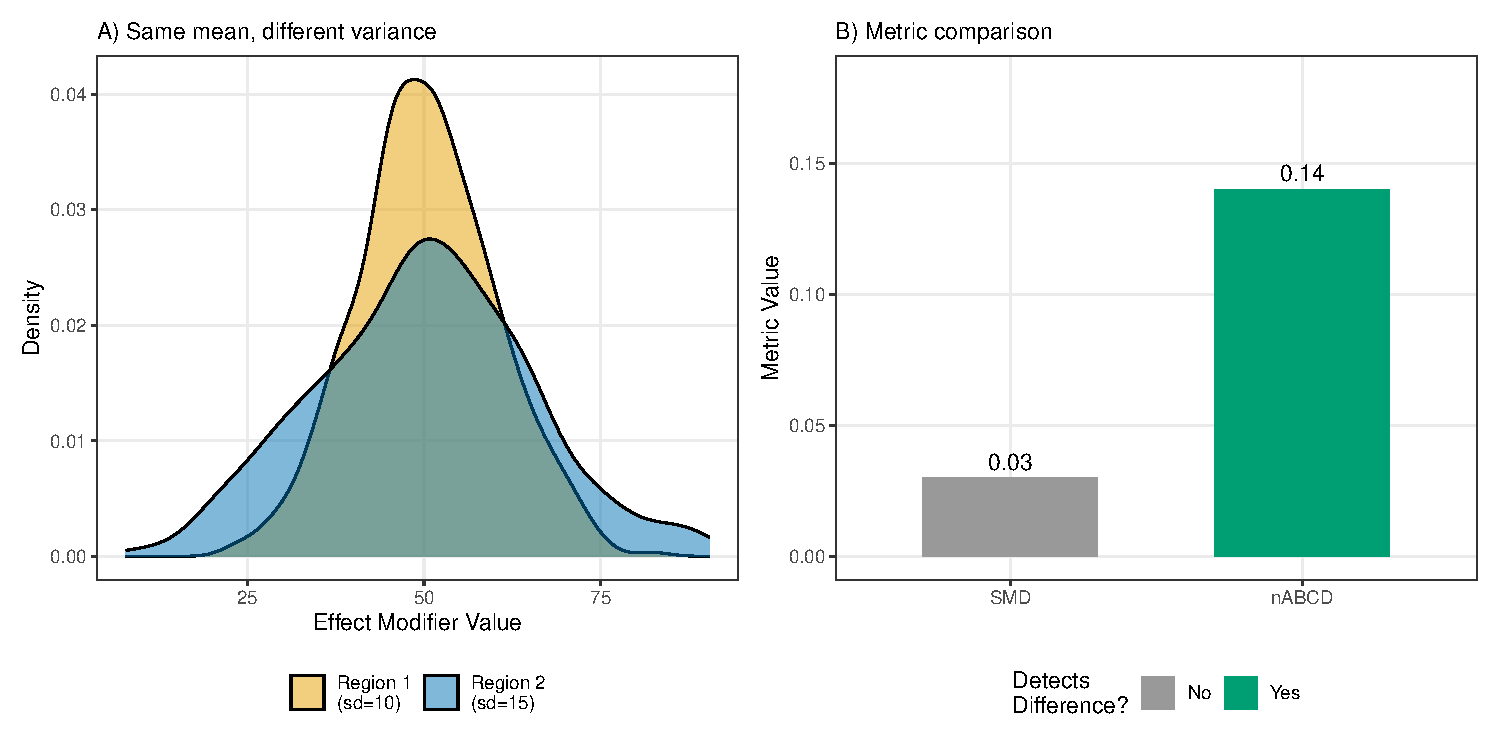
\includegraphics[width=\textwidth]{fig5_smd_comparison.pdf}}
\caption{Comparison of nABCD and SMD across distributional difference types. nABCD responds to scale (S5) and shape (S6) differences where SMD remains near zero, demonstrating its advantage for full distributional comparison.\label{fig:smd}}
\end{figure*}

In summary, the simulation study across eight scenarios demonstrates that the nABCD estimator provides reliable estimation with the following properties at sample sizes typical in MRCT regional subgroups:
\begin{enumerate}[1.]
\item \emph{Bias}: Less than 0.02 for most non-null scenarios at $n \geq 100$; positive bias is largest near the boundary (S1: 0.065, S6: 0.046 at $n = 100$) and negligible for scenarios with true nABCD above 0.1 (S3: 0.003, S4: 0.003 at $n = 100$)
\item \emph{Coverage}: 0.88--0.96 at $n \geq 100$ for scenarios with true nABCD $\geq 0.1$ (S3--S5, S7, S8); S7 (skew) and S8 (location + scale) achieved coverage between 0.93--0.95
\item \emph{Precision}: RMSE below 0.06 and CI width below 0.19 at $n \geq 100$
\item \emph{Sensitivity}: Captures location, scale, and shape differences where SMD is limited to location only
\end{enumerate}

Scenario S3 (0.5$\sigma$ location shift, true nABCD $= 0.180$) exemplifies the operating characteristics at clinically relevant effect sizes: bias was negligible ($+0.003$ at $n = 100$), coverage was nominal (0.951), and CI width (0.18) translated to a $\Delta_{\max}$ CI width of $2 \times 0.01 \times 11 \times 0.18 = 0.040$ (4.0\%pt) when calibrated with $L = 0.01$/pt and IQR $= 11$ (NIHSS-scale parameters)---a level of precision sufficient for informed regulatory deliberation.

These estimation properties ensure that nABCD, when combined with the clinical calibration framework, provides $\Delta_{\max}$ estimates of sufficient quality for regulatory deliberation. We recommend $n \geq 100$ per region for reliable estimation and inference.

%==============================================================================
\section{Application: Hypothetical Thrombolytic MRCT Using GUSTO-I Data}\label{sec:application}
%==============================================================================

We illustrate the nABCD framework through a hypothetical scenario grounded in publicly available data from GUSTO-I, a large international trial in acute myocardial infarction (AMI). A sponsor is developing a novel thrombolytic agent (Drug~T) for AMI and is planning a Phase~3 MRCT across multiple regions. At the planning stage, the sponsor uses publicly available individual patient data (IPD) from GUSTO-I ($N = 40{,}830$; 16 anonymized regions)\cite{gusto1993} to assess distributional similarity of candidate effect modifiers across regions and to identify suitable pooling partners for a designated anchor region.

\subsection{Scenario Design and Effect Modifier Selection}\label{sec:app_scenario}

The FTT Collaborative Group\cite{ftt1994} meta-analysis of fibrinolytic therapy trials established age as a confirmed effect modifier for thrombolytic efficacy in AMI: the absolute mortality reduction varied from approximately 1\%pt in patients aged $<55$ to 3.4\%pt in those aged 55--74, declining to non-significant in patients aged $\geq75$. From these published subgroup-specific treatment effects, CATE sensitivity is estimable: $L_{\text{mean}} = 0.0003$/yr and $L_{\max} = 0.0005$/yr. Systolic blood pressure (SBP) was also examined in FTT as a candidate effect modifier, but the treatment $\times$ SBP interaction evidence is weaker and $L$ is not directly estimable from the published data. These two candidate effect modifiers represent complementary planning scenarios: age permits clinical calibration via $\Delta_{\max}$ (equation~\ref{eq:delta_max}), while SBP requires $L^*$ sensitivity analysis (equation~\ref{eq:lstar}).

The sponsor selects Region~8 as the anchor region---representing, for instance, a regulatory market where local efficacy evidence is required but sample size is limited. Region~8 enrolled $n = 2{,}916$ patients, with baseline characteristics summarized in Table~\ref{tab:gusto_r8}. The exercise of identifying Region~8's suitable pooling partners simulates the decision a sponsor would face when seeking regional efficacy assessment through pooling under ICH E17.\cite{iche17}

\begin{table}[ht]
\caption{Region~8 baseline characteristics (GUSTO-I).\label{tab:gusto_r8}}
\begin{tabular*}{\textwidth}{@{\extracolsep\fill}lcccc@{}}
\toprule
\textbf{Effect modifier} & \textbf{Mean} & \textbf{SD} & \textbf{Skewness} & \textbf{IQR\textsubscript{pooled}} \\
\midrule
Age (years) & 60.2 & 12.1 & $-0.17$ & 17--18 \\
SBP (mmHg) & 132.4 & 22.9 & 0.20 & 30--34 \\
\bottomrule
\end{tabular*}
\begin{tablenotes}
\item $n = 2{,}916$. IQR\textsubscript{pooled} ranges reflect variation across the 15 partner-region pairs.
\end{tablenotes}
\end{table}

\subsection{Distributional Assessment: nABCD Across 15 Partner Regions}\label{sec:app_nabcd}

We computed nABCD between Region~8 and each of the remaining 15 regions for both candidate effect modifiers, with percentile bootstrap 95\% confidence intervals ($B = 2{,}000$). Table~\ref{tab:gusto_nabcd} presents the results, ranked by nABCD for age. Figure~\ref{fig:gusto_forest} displays these results as a forest plot with bootstrap CIs.

\begin{table}[ht]
\caption{nABCD values (with 95\% percentile bootstrap CIs) for Region~8 versus each partner region (GUSTO-I).\label{tab:gusto_nabcd}}
\begin{tabular*}{\textwidth}{@{\extracolsep\fill}lrlcrlc@{}}
\toprule
 & \multicolumn{3}{c}{\textbf{Age}} & \multicolumn{3}{c}{\textbf{SBP}} \\
\cmidrule{2-4} \cmidrule{5-7}
\textbf{Partner} & $n$ & \textbf{nABCD [95\% CI]} & \textbf{Pool?} & \textbf{nABCD [95\% CI]} & \textbf{Pool?} & \textbf{Joint} \\
\midrule
R5  & 1909 & 0.011 [0.010, 0.026] & Y & 0.056 [0.038, 0.077] & N & N \\
R7  & 3150 & 0.011 [0.008, 0.026] & Y & 0.082 [0.064, 0.098] & N & N \\
R4  & 2876 & 0.016 [0.010, 0.032] & Y & 0.042 [0.029, 0.060] & Y & Y \\
R9  & 3123 & 0.017 [0.011, 0.032] & Y & 0.110 [0.091, 0.130] & N & N \\
R15 & 2576 & 0.017 [0.011, 0.034] & Y & 0.074 [0.057, 0.093] & N & N \\
R1  & 2188 & 0.018 [0.014, 0.028] & Y & 0.058 [0.044, 0.079] & N & N \\
R14 & 3437 & 0.020 [0.012, 0.036] & Y & 0.064 [0.052, 0.082] & N & N \\
R12 & 4352 & 0.024 [0.013, 0.040] & Y & 0.097 [0.083, 0.117] & N & N \\
R6  & 1585 & 0.026 [0.018, 0.040] & Y & 0.050 [0.032, 0.076] & Y$^{\dagger}$ & Y$^{\dagger}$ \\
R13 & 2297 & 0.034 [0.022, 0.051] & Y & 0.037 [0.023, 0.061] & Y & Y \\
R11 & 2491 & 0.035 [0.021, 0.052] & Y & 0.104 [0.082, 0.122] & N & N \\
R10 & 1717 & 0.038 [0.022, 0.058] & Y & 0.062 [0.045, 0.085] & N & N \\
R16 & 1231 & 0.050 [0.034, 0.071] & N$^{\ddagger}$ & 0.071 [0.051, 0.095] & N & N \\
R2  & 2952 & 0.061 [0.044, 0.079] & N & 0.015 [0.012, 0.030] & Y & N \\
R3  & 2030 & 0.076 [0.057, 0.095] & N & 0.051 [0.035, 0.074] & N & N \\
\bottomrule
\end{tabular*}
\begin{tablenotes}
\item Poolability determined by nABCD $< 0.05$. Y = poolable; N = not poolable. Regions ranked by age nABCD (ascending). Bootstrap: $B = 2{,}000$, seed = 2026.
\item[$\dagger$] R6: nABCD(SBP) $= 0.0496$, marginally below the 0.05 threshold; the 95\% CI $[0.032, 0.076]$ spans both sides.
\item[$\ddagger$] R16: nABCD(age) $= 0.0504$, marginally above the 0.05 threshold; the 95\% CI $[0.034, 0.071]$ spans both sides.
\end{tablenotes}
\end{table}

\begin{figure}[ht]
\centering

\includegraphics[width=\textwidth]{figures/fig_gusto_r8_forest}
\caption{Forest plot of nABCD with 95\% percentile bootstrap CIs for Region~8 versus each partner region, for age (left) and systolic blood pressure (right). The dashed vertical line indicates the nABCD $= 0.05$ threshold. Blue = poolable; orange = boundary; red = not poolable.}
\label{fig:gusto_forest}
\end{figure}

The two effect modifiers produce strikingly different poolability patterns. For age, 12 of 15 partner regions satisfy the $\text{nABCD} < 0.05$ threshold, with point estimates ranging from 0.011 (R5, R7) to 0.038 (R10). R16 ($\text{nABCD} = 0.050$) falls at the boundary, while R2 (0.061) and R3 (0.076) clearly exceed it. For SBP, only 4 of 15 regions have point estimates below 0.05: R2 (0.015), R13 (0.037), R4 (0.042), and R6 (0.050); the remaining 11 regions range from 0.056 (R5) to 0.110 (R9). The higher SBP nABCD values across most regions reflect greater geographic heterogeneity in blood pressure distributions compared to age.

Two boundary cases merit discussion. R16 has $\text{nABCD}(\text{age}) = 0.050$, placing it at the threshold; its 95\% CI $[0.034, 0.071]$ spans both sides, leaving poolability indeterminate from a statistical standpoint. R6 has $\text{nABCD}(\text{SBP}) = 0.050$, also near the threshold; its 95\% CI $[0.032, 0.076]$ similarly does not resolve the classification. These cases illustrate the value of reporting bootstrap CIs alongside point estimates: the binary poolable/not-poolable determination is supplemented by the uncertainty interval, which informs the degree of confidence in the classification.

An instructive contrast emerges between R2 and R9: R2 has the second-largest age nABCD (0.061) but the smallest SBP nABCD (0.015), while R9 has the second-smallest age nABCD (0.017) but the largest SBP nABCD (0.110). A pooling decision based on either effect modifier alone would reach opposite conclusions for these regions. This underscores the necessity of evaluating all candidate effect modifiers jointly, as visualized in Figure~\ref{fig:gusto_scatter}.

\begin{figure}[ht]
\centering

\includegraphics[width=\textwidth]{figures/fig_gusto_r8_scatter}
\caption{Joint pooling assessment for Region~8. Each point represents a partner region, positioned by nABCD for age (horizontal) and SBP (vertical). Dashed lines at nABCD $= 0.05$ create four quadrants. The shaded lower-left quadrant contains regions poolable for both effect modifiers (R4, R6, R13). R2 is poolable for SBP only; many regions are poolable for age only.}
\label{fig:gusto_scatter}
\end{figure}

\subsection{Clinical Calibration: Age}\label{sec:app_age}

Because age is a confirmed effect modifier with estimable CATE sensitivity, clinical calibration translates the observed nABCD values into treatment effect heterogeneity on the clinical outcome scale. Using the FTT-derived estimates ($L_{\text{mean}} = 0.0003$/yr, $L_{\max} = 0.0005$/yr) and equation~(\ref{eq:delta_max}):
\[
\Delta_{\max} = 2L \cdot \text{IQR}_{\text{pooled}} \cdot \text{nABCD}.
\]

Table~\ref{tab:gusto_delta} presents $\Delta_{\max}$ for selected region pairs, using pair-specific $\text{IQR}_{\text{pooled}}$ values (range: 17.0--18.4 years).

\begin{table}[ht]
\caption{Clinical calibration ($\Delta_{\max}$) for age: Region~8 versus selected partners.\label{tab:gusto_delta}}
\begin{tabular*}{\textwidth}{@{\extracolsep\fill}lccccc@{}}
\toprule
\textbf{Partner} & \textbf{nABCD} & \textbf{IQR\textsubscript{pooled}} & \multicolumn{2}{c}{\textbf{$\Delta_{\max}$ (\%pt)}} & \textbf{Pool?} \\
\cmidrule{4-5}
 & & (years) & $L_{\text{mean}}$ & $L_{\max}$ & \\
\midrule
R5  & 0.011 & 17.8 & 0.012 & 0.019 & Y \\
R4  & 0.016 & 17.9 & 0.017 & 0.028 & Y \\
R13 & 0.034 & 17.0 & 0.034 & 0.057 & Y \\
R6  & 0.026 & 17.2 & 0.027 & 0.046 & Y \\
R16 & 0.050 & 17.3 & 0.052 & 0.087 & N$^{\ddagger}$ \\
R2  & 0.061 & 17.6 & 0.064 & 0.107 & N \\
R3  & 0.076 & 17.2 & 0.078 & 0.130 & N \\
\bottomrule
\end{tabular*}
\begin{tablenotes}
\item $\Delta_{\max}$ computed as $2L \times \text{IQR}_{\text{pooled}} \times \text{nABCD}$. FTT-derived estimates: $L_{\text{mean}} = 0.0003$/yr, $L_{\max} = 0.0005$/yr.
\item[$\ddagger$] R16: nABCD at boundary ($= 0.050$).
\end{tablenotes}
\end{table}

For the maximum-nABCD pair (Region~8--R3, $\text{nABCD} = 0.076$):
\begin{itemize}
  \item Using $L_{\max} = 0.0005$/yr: $\Delta_{\max} = 2 \times 0.0005 \times 17.2 \times 0.076 = 0.13$\%pt.
  \item Using $L_{\text{mean}} = 0.0003$/yr: $\Delta_{\max} = 2 \times 0.0003 \times 17.2 \times 0.076 = 0.08$\%pt.
\end{itemize}
These values are negligible relative to the overall treatment effect of thrombolytic therapy in AMI (approximately 2--3\%pt absolute mortality reduction in FTT). Even the non-poolable pair with the largest distributional difference produces a worst-case treatment effect heterogeneity below 0.13\%pt. For the jointly poolable regions, $\Delta_{\max}$ values are smaller still: R13 ($\text{nABCD} = 0.034$) yields $\Delta_{\max} = 0.057$\%pt under $L_{\max}$. Figure~\ref{fig:gusto_calibration}(a) displays the full $\Delta_{\max}$ profile across all 15 partners.

The clinical calibration confirms that age distributional differences across GUSTO-I regions are unlikely to generate clinically meaningful treatment effect heterogeneity for Drug~T, even under conservative assumptions about CATE sensitivity.

\subsection{Sensitivity Analysis: SBP}\label{sec:app_sbp}

Because $L$ for SBP is not estimable from published data, we conduct $L^*$ reverse-calculation analysis (equation~\ref{eq:lstar}) to determine what CATE sensitivity would be required for the observed distributional differences to produce clinically meaningful heterogeneity. Using pair-specific $\text{IQR}_{\text{pooled}}$ values (range: 30--34~mmHg):
\[
L^* = \frac{\Delta_{\text{clin}}}{2 \cdot \text{IQR}_{\text{pooled}} \cdot \text{nABCD}}.
\]

For the maximum-nABCD pair (Region~8--R9, $\text{nABCD} = 0.110$, $\text{IQR}_{\text{pooled}} = 31$~mmHg):
\begin{itemize}
  \item At $\Delta_{\text{clin}} = 1$\%pt: $L^* = 0.01 / (2 \times 31 \times 0.110) = 0.0015$/mmHg.
  \item At $\Delta_{\text{clin}} = 2$\%pt: $L^* = 0.02 / (2 \times 31 \times 0.110) = 0.0029$/mmHg.
\end{itemize}

A CATE sensitivity of $L = 0.0015$/mmHg means that the treatment effect changes by 0.15\%pt for every 1~mmHg change in baseline SBP---a modest value that cannot be ruled out based on published evidence. This suggests that SBP distributional differences between Region~8 and non-poolable partners could plausibly translate into clinically meaningful heterogeneity if a treatment $\times$ SBP interaction exists for Drug~T. Even for pairs closer to the threshold (e.g., R5 with $\text{nABCD} = 0.056$, $\text{IQR}_{\text{pooled}} = 30$~mmHg), $L^* = 0.0030$/mmHg at $\Delta_{\text{clin}} = 1$\%pt---still within a plausible range. Figure~\ref{fig:gusto_calibration}(b) displays the $L^*$ profile across SBP-non-poolable partners.

This sensitivity analysis does not prove that SBP distributional differences will produce treatment effect heterogeneity; rather, it quantifies the conditions under which they would. The modest $L^*$ values indicate that the distributional heterogeneity detected by nABCD warrants explicit consideration in the pooling strategy, even without confirmed effect modifier evidence for SBP.

\begin{figure}[ht]
\centering

\includegraphics[width=\textwidth]{figures/fig_gusto_r8_calibration}
\caption{Clinical interpretation of nABCD values for Region~8. (a)~Age: $\Delta_{\max}$ under two CATE sensitivity assumptions ($L_{\text{mean}} = 0.0003$/yr, $L_{\max} = 0.0005$/yr) for all 15 partner regions, ordered by nABCD. (b)~SBP: $L^*$ (minimum CATE sensitivity to produce $\Delta_{\text{clin}}$) at two clinical thresholds ($\Delta_{\text{clin}} = 1$\%pt, 2\%pt) for the 11 SBP-non-poolable partner regions.}
\label{fig:gusto_calibration}
\end{figure}

\subsection{Pooling Recommendation}\label{sec:app_pooling}

When multiple candidate effect modifiers are evaluated, a region qualifies as a pooling partner only if it satisfies the similarity criterion for every effect modifier---the most restrictive condition governs. Combining the age and SBP assessments:

\begin{itemize}
  \item \textbf{Age}: 12 of 15 regions poolable ($\text{nABCD} < 0.05$); R16 ($\text{nABCD} = 0.050$) falls at the boundary.
  \item \textbf{SBP}: 4 of 15 regions have $\text{nABCD} < 0.05$: R2 (0.015), R13 (0.037), R4 (0.042), and R6 (0.050); R6 is near the boundary ($\text{nABCD} = 0.0496$, 95\% CI $[0.032, 0.076]$).
  \item \textbf{Both effect modifiers}: 3 regions satisfy both criteria---R4, R6, and R13---constituting Region~8's pooling group.
\end{itemize}

R2 is poolable for SBP ($\text{nABCD} = 0.015$) but not for age ($\text{nABCD} = 0.061$); conversely, many regions poolable for age (e.g., R9 with $\text{nABCD}_{\text{age}} = 0.017$) are excluded by SBP ($\text{nABCD}_{\text{SBP}} = 0.110$). This pattern illustrates a central practical implication: the number of eligible pooling partners depends critically on how many effect modifiers are assessed and on the distributional heterogeneity specific to each. In this scenario, SBP---the effect modifier with weaker prior evidence but greater geographic heterogeneity---is the binding constraint.

The R6 boundary case ($\text{nABCD}(\text{SBP}) = 0.0496$) warrants transparent reporting. The point estimate falls marginally below 0.05, but the 95\% CI $[0.032, 0.076]$ encompasses both poolable and non-poolable classifications. Under a strict $< 0.05$ criterion, R6 qualifies; the estimation-centered approach recommends reporting the full CI and $\Delta_{\max}$ (once $L$ becomes available) rather than relying solely on the binary classification. Similarly, R16's $\text{nABCD}(\text{age}) = 0.050$ illustrates that threshold-based decisions at the boundary benefit from the additional information provided by the bootstrap CI and clinical calibration.

The practical consequence for the sponsor is threefold. First, the three confirmed partners (R4, R6, R13) can be designated as Region~8's pooling group for regulatory assessment, with the caveat that R6's SBP classification carries uncertainty. Second, the clinical calibration for age demonstrates that the age-based exclusions (R16, R2, R3) have negligible clinical impact ($\Delta_{\max} < 0.13$\%pt); the substantive pooling constraint arises from SBP distributional differences. Third, if the sponsor obtains additional evidence on SBP---for example, from a Phase~2 interaction analysis or an external database---that evidence can be incorporated through the clinical calibration framework: estimating $L$ for SBP would allow direct $\Delta_{\max}$ computation, potentially expanding or narrowing the pooling set with clinical justification.

Several limitations of this application should be noted:
\begin{enumerate}[1.]
\item \emph{Illustrative data source}: GUSTO-I was not designed as an MRCT; it serves as a convenient publicly available data source for methodological demonstration. In practice, sponsors would assemble regional effect modifier distributions from the most representative and current sources available.
\item \emph{Anonymized regions}: GUSTO-I regions are anonymized, precluding demographic or geographic interpretation of the distributional patterns. This limitation is specific to the dataset, not the framework.
\item \emph{Transferability of $L$}: CATE sensitivity for age was estimated from the FTT meta-analysis of first-generation thrombolytics; the class-transferability assumption to Drug~T requires justification and sensitivity analysis.
\item \emph{Threshold choice}: The $\text{nABCD} < 0.05$ threshold used here is illustrative. In practice, threshold selection should reflect clinical context, regulatory requirements, and the clinical calibration results. The estimation-centered approach (reporting $\Delta_{\max}$ with CIs) provides richer information than a binary poolable/not-poolable determination.
\end{enumerate}

%==============================================================================
\section{Discussion}\label{sec:discussion}
%==============================================================================

We developed nABCD, a normalized dissimilarity index that combines Wasserstein-1 distance with IQR normalization to capture full distributional differences---including scale, shape, and skewness---that conventional measures such as SMD miss. The clinical calibration framework translates these distributional differences into context-specific $\Delta_{\max}$ assessments when CATE sensitivity $L$ is estimable. The IST-3 application demonstrated a key practical implication: rankings by distributional magnitude and clinical impact can diverge---age exhibited the largest nABCD ($0.285$) yet smallest $\Delta_{\max}$ ($0.47$\%pt), while NIHSS showed moderate nABCD ($0.240$) but substantially larger $\Delta_{\max}$ ($5.02$\%pt)---underscoring that clinical calibration, not nABCD magnitude alone, should guide pooling decisions.

Compared to existing approaches, nABCD offers three advantages. First, it captures distributional differences invisible to SMD: our simulation confirmed that scale (S5), shape (S6), and skewness (S7) differences produced near-zero SMD but non-negligible nABCD, and the IST-3 application revealed the same pattern with real data (treatment delay: SMD $\approx 0$ between Norway and Portugal, nABCD $= 0.069$). Second, unlike the KS statistic, nABCD connects directly to treatment effect heterogeneity through the heterogeneity bound (equation~\ref{eq:delta_max}), enabling clinical calibration rather than purely statistical assessment. Third, unlike visual inspection, nABCD is objective, reproducible, and amenable to bootstrap inference. Our approach is conceptually distinct from treatment effect consistency assessment methods\cite{quan2010} which evaluate whether observed treatment effects agree across regions; nABCD operates upstream, quantifying similarity in the effect modifier distributions that may drive such heterogeneity.

The clinical calibration procedure introduced in Section~\ref{sec:inference} represents a departure from fixed-threshold approaches. Cohen's $d$ benchmarks (small = 0.2, medium = 0.5, large = 0.8) have been widely criticized for context-free application, and we deliberately avoid this pattern. Instead, the heterogeneity bound provides a principled mechanism to translate nABCD into clinically meaningful units, respecting the ICH E17 principle that ``similar enough'' is context-dependent. A natural consequence of clinical calibration is that rankings by distributional distance and clinical impact may differ---as observed in IST-3, where age had the largest nABCD yet the smallest $\Delta_{\max}$---because the same distributional difference carries different clinical weight depending on CATE sensitivity. More broadly, the IST-3 application demonstrated that the same nABCD framework serves different purposes depending on the availability of CATE sensitivity evidence: for NIHSS, where $L$ was estimable, full calibration translated distributional differences into clinically interpretable $\Delta_{\max}$ values; for age, where $L$ was uncertain, nABCD with reference benchmarks (Table~\ref{tab:benchmarks}) provided the primary assessment of distributional similarity. This connection draws on transportability theory\cite{pearl2011,bareinboim2016} to relate distributional distance to potential treatment effect heterogeneity.

Based on our findings, we offer the following recommendations for practitioners:
\begin{enumerate}[1.]
\item Compute nABCD with bootstrap CIs ($n \geq 100$ per region) for each candidate effect modifier across region pairs.
\item Translate nABCD into $\Delta_{\max}$ and its CI on the clinical outcome scale using equation~(\ref{eq:delta_max}), incorporating prior knowledge or estimates of CATE sensitivity $L$. When $L$ is estimated from data, report both $L_{\max}$ (conservative upper bound) and $L_{\text{mean}}$ (realistic estimate), as in the IST-3 application (Section~\ref{sec:application}).
\item Report $\Delta_{\max}$ and its CI alongside the overall treatment effect, non-inferiority margin, or other clinically relevant benchmarks to support informed deliberation about pooling.
\item Conduct sensitivity analyses over plausible values of $L$ when prior knowledge is uncertain.
\item When $L$ cannot be estimated, use the reference benchmarks in Table~\ref{tab:benchmarks} as initial guidance, recognizing that clinical calibration provides a more rigorous basis for decision-making.
\end{enumerate}

In practice, multiple candidate effect modifiers may be evaluated simultaneously. The nABCD framework assesses each effect modifier separately, and we recommend reporting $\Delta_{\max}$ and its CI for every candidate effect modifier across all region pairs. To arrive at an overall pooling recommendation, trial designers may adopt a conservative approach based on the maximum $\Delta_{\max}$ across all effect modifiers and region pairs, or they may take a totality-of-evidence approach in which the collection of $\Delta_{\max}$ values, together with their uncertainties and the reliability of each $L$ estimate, informs a holistic judgment. The choice between these strategies depends on the regulatory context: for applications where a formal pooling criterion is required, the maximum $\Delta_{\max}$ provides a defensible worst-case assessment; for advisory settings where pooling decisions are informed by clinical deliberation, the full set of calibrated results offers a richer evidence base.

A distinctive practical advantage of the nABCD framework is its compatibility with diverse data sources. Because nABCD requires only baseline effect modifier distributions---not treatment outcomes---regional distributional data can be assembled from prior clinical trials, disease registries, electronic health records, epidemiological databases, or other real-world evidence (RWE) sources. This data-source flexibility is increasingly relevant as regulatory agencies promote the use of RWE in drug development (ICH E6(R3)). The representativeness of the data source with respect to the target trial population is a prerequisite for valid nABCD estimation, regardless of the data origin.

\emph{Application to Japanese and Chinese regulatory contexts.} The nABCD framework is particularly relevant for regulatory submissions requiring regional subpopulation consistency.\cite{matsushima2024,song2025} In global MRCTs, regional enrolment is often limited, making direct demonstration of consistency difficult. Matsushima et al.'s\cite{matsushima2024} PMDA workshop documented that regional imbalance in CRP-positive/MRI-negative status caused apparent inconsistency in the secukinumab MRCT, underscoring the practical consequences when effect modifier distributional differences are not assessed at the planning stage. nABCD provides the quantitative tool to identify such distributional differences prospectively, enabling sponsors to select pooling partners that minimize the risk of apparent inconsistency. As demonstrated in the IST-3 application using Belgium ($n=73$) as a small-sample anchor, the framework directly simulates the decision environment faced by sponsors seeking regulatory-compliant regional assessment through pooling.

The practical availability of CATE sensitivity $L$ varies across settings. When $L$ is estimable from prior trials or meta-analyses in the same therapeutic area, full clinical calibration is possible, as demonstrated for NIHSS in the IST-3 application. At the MRCT planning stage, however, $L$ is often uncertain---particularly for novel agents or therapeutic areas lacking subgroup analyses. In such cases, nABCD with reference benchmarks (Table~\ref{tab:benchmarks}) provides the primary assessment of distributional similarity, supplemented by sensitivity analysis over plausible $L$ ranges. Importantly, nABCD's core value as a distributional measure---capturing scale, shape, and skewness differences invisible to SMD---holds regardless of whether $L$ is available; clinical calibration enhances but does not replace this distributional assessment.

Several limitations should be acknowledged:
\begin{enumerate}[1.]
\item The current formulation applies to continuous effect modifiers only; extensions to categorical or mixed-type effect modifiers require further development.
\item nABCD evaluates each effect modifier separately rather than jointly; a multivariate extension would address potential confounding among effect modifiers.
\item Positive bias under the null and near-boundary scenarios (true nABCD $\lesssim 0.05$) can inflate nABCD estimates and prevent nominal coverage. This is inherent to the non-negative nature of nABCD as a function of the Wasserstein distance: when the true value lies at or near the boundary of the parameter space, sampling variability produces strictly positive estimates even when the true distributional difference is negligible.\cite{andrews2000} In our simulation, S6 (shape; true nABCD $= 0.024$) exhibited substantial positive bias (0.071 at $n=50$, 0.028 at $n=200$) and zero coverage at all sample sizes. We therefore do not report coverage for near-boundary scenarios and recommend interpreting nABCD estimates near zero with caution. For scenarios with true nABCD above approximately 0.1, the parameter lies in the interior of the parameter space where standard bootstrap consistency holds, and our simulation confirms this with coverage of 0.88--0.96 at $n \geq 100$ across S2--S5, S7, and S8; S4 (1.0$\sigma$ location shift; true nABCD $= 0.328$) achieved near-nominal coverage (0.950--0.957), confirming reliable inference even for large distributional differences. We use the percentile bootstrap, which is first-order accurate; bias-corrected methods such as BCa showed inferior performance for this bounded statistic (Section~\ref{sec:sim_results}), and the studentized bootstrap would require variance estimation for the Wasserstein distance ratio, which adds substantial complexity. We recommend $n \geq 100$ per region for reliable point estimation and confidence intervals.
\item The clinical calibration requires estimation of CATE sensitivity $L$, which may not always be available from prior data. Reference benchmarks are provided as a fallback but should not replace context-specific calibration.
\item When multiple effect modifiers are relevant, the current framework evaluates each separately. Aggregation strategies for combining nABCD values across effect modifiers---such as weighted combinations reflecting clinical importance or multivariate extensions using higher-dimensional optimal transport---remain topics for future investigation.
\item As with any covariate-based approach, nABCD assesses similarity only with respect to measured effect modifiers. Unmeasured or unknown effect modifiers may contribute to treatment effect heterogeneity beyond what the index captures.
\item The clinical calibration demonstrated in the IST-3 application used CATE sensitivity estimates from alteplase; transferability of $L$ to other agents in the same pharmacological class is an assumption that requires clinical judgment and may benefit from sensitivity analysis.
\item The IST-3 data were collected during 2000--2011; demographic and clinical practice changes may limit the applicability of these country-level effect modifier distributions to contemporary trial planning.
\end{enumerate}

Future work should address multivariate extensions, bias correction methods for small samples, and empirical calibration of CATE sensitivity parameters using real MRCT data. Methods for estimating $L$ from historical trial databases would strengthen the clinical calibration framework. The nABCD framework could also be extended to longitudinal effect modifier profiles, enabling dynamic assessment of distributional similarity over time.

An R package implementing the nABCD index with bootstrap inference and the clinical calibration framework described herein is under development.

nABCD fills a methodological gap in ICH E17 implementation by providing a principled framework for assessing distributional similarity. Rather than reducing ``similar enough'' to a fixed threshold, the clinical calibration procedure translates distributional differences into context-specific assessments of potential treatment effect heterogeneity, enabling evidence-based and clinically grounded pooling decisions. Open-source R code is available to facilitate adoption.

%==============================================================================
% Back matter
%==============================================================================

\bmsection*{Author contributions}

[Author 1] conceived the research question and led the project. [Author 2] developed the mathematical framework and conducted the simulation study. [Author 3] contributed to the application example and manuscript preparation. All authors reviewed and approved the final manuscript.

\bmsection*{Acknowledgments}

The authors thank [colleagues] for helpful discussions on ICH E17 implementation.

\bmsection*{Financial disclosure}

None reported.

\bmsection*{Conflict of interest}

The authors declare no potential conflict of interests.

\bmsection*{Data availability statement}

R code for computing nABCD and reproducing the simulation study is available at [repository URL]. The IST-3 individual patient data are publicly available from Edinburgh DataShare.\cite{ist3_2012}

\bibliography{nABCD_wiley}

\bmsection*{Supporting information}

Additional supporting information may be found in the online version of the article at the publisher's website. Supporting materials include: complete R code for nABCD computation, simulation scripts, and additional figures for realistic clinical scenarios.

%==============================================================================
\appendix
%==============================================================================

\bmsection{Proofs and Mathematical Details\label{app:proofs}}

\bmsubsection{Proof of Proposition~\ref{prop:nonnegativity}\label{app:proof1}}

Non-negativity follows directly from the non-negativity of the Wasserstein-1 distance: $W_1(F_1, F_2) = \int |F_1(x) - F_2(x)| \, dx \geq 0$. Since $\text{IQR}_{\text{pooled}} > 0$ for non-degenerate distributions, the ratio $\text{nABCD} = W_1 / (2 \cdot \text{IQR}_{\text{pooled}}) \geq 0$.

For the identity of indiscernibles, we show both directions. If $F_1 = F_2$, then $|F_1(x) - F_2(x)| = 0$ for all $x$, so $W_1(F_1, F_2) = 0$ and hence $\text{nABCD} = 0$. Conversely, if $\text{nABCD} = 0$, then $W_1(F_1, F_2) = \int |F_1(x) - F_2(x)| \, dx = 0$. Since $|F_1(x) - F_2(x)| \geq 0$ and is right-continuous, $\int |F_1(x) - F_2(x)| \, dx = 0$ implies $F_1(x) = F_2(x)$ almost everywhere; by right-continuity of CDFs, $F_1 = F_2$ everywhere.

\bmsubsection{Asymptotic Properties\label{app:asymptotic}}

Under standard regularity conditions, the empirical Wasserstein-1 distance $W_1(\hat{F}_1, \hat{F}_2)$ is a consistent estimator of $W_1(F_1, F_2)$.\cite{delbarrio1999} Combined with the consistency of the empirical IQR, $\hnABCD$ is a consistent estimator of $\text{nABCD}(F_1, F_2)$.

In one dimension, the empirical $W_1$ distance converges at rate $O(n^{-1/2})$ without logarithmic correction.\cite{delbarrio1999} For two-sample estimation with $F_1 \neq F_2$ and finite second moments, $\sqrt{n}(W_1(\hat{F}_{1,n_1}, \hat{F}_{2,n_2}) - W_1(F_1, F_2))$ converges in distribution to a mean-zero Gaussian, where $n = n_1 + n_2$ with $n_1/n \to \lambda \in (0,1)$. Since the empirical IQR also converges at rate $O(n^{-1/2})$ under standard density conditions, the delta method applied to the ratio $g(w, q) = w/(2q)$ yields asymptotic normality of $\hnABCD$:
\begin{equation}
\sqrt{n}\bigl(\hnABCD - \text{nABCD}(F_1, F_2)\bigr) \xrightarrow{d} N(0,\, \sigma^2_{\text{nABCD}}),
\label{eq:asymptotic_normality}
\end{equation}
where $\sigma^2_{\text{nABCD}}$ depends on the asymptotic variances and covariance of the $W_1$ and IQR estimators. This result requires $\text{nABCD} > 0$ (i.e., $F_1 \neq F_2$); at the boundary $F_1 = F_2$, the parameter lies on the edge of the parameter space and standard asymptotics do not apply (see Section~\ref{sec:discussion}).

The bootstrap provides valid inference for the Wasserstein distance under mild conditions.\cite{sommerfeld2018} The percentile bootstrap confidence interval achieves asymptotically correct coverage for non-degenerate distributions.

\bmsection{R Code for nABCD Computation\label{app:rcode}}

\begin{lstlisting}[caption={R function for computing nABCD with bootstrap confidence intervals.},label=lst:nabcd,basicstyle=\fontsize{8}{10}\selectfont\ttfamily]
compute_nABCD <- function(x1, x2) {
  pooled <- c(x1, x2)
  iqr_pooled <- IQR(pooled)
  if (iqr_pooled == 0) return(NA)
  all_vals <- sort(unique(pooled))
  F1 <- ecdf(x1); F2 <- ecdf(x2)
  w1 <- sum(diff(all_vals) *
    abs(F1(all_vals[-length(all_vals)]) -
        F2(all_vals[-length(all_vals)])))
  w1 / (2 * iqr_pooled)
}

nABCD_bootstrap <- function(x1, x2,
    B = 2000, conf = 0.95) {
  obs <- compute_nABCD(x1, x2)
  boot_vals <- replicate(B, {
    b1 <- sample(x1, replace = TRUE)
    b2 <- sample(x2, replace = TRUE)
    compute_nABCD(b1, b2)
  })
  alpha <- 1 - conf
  ci <- quantile(boot_vals,
    c(alpha/2, 1 - alpha/2), na.rm = TRUE)
  list(estimate = obs,
       ci_lower = ci[1], ci_upper = ci[2])
}
\end{lstlisting}

\end{document}
